\documentclass{article}

% Basic packages
\usepackage[a4paper, margin=2cm]{geometry}
\usepackage{tikz}
\usetikzlibrary{calc, positioning, external, fit}
\tikzexternalize[prefix=figs/,optimize command away=\includepdf]
\tikzset{
	vector/.style = {#1, ultra thick, -stealth, cap=round},
}
\usepackage{hyperref}

% Colors
\definecolor{xred}{HTML}{BD4242}
\definecolor{xblue}{HTML}{4268BD}
\definecolor{xgreen}{HTML}{52B256}
\definecolor{xpurple}{HTML}{7F52B2}
\definecolor{xorange}{HTML}{FD9337}

% General defs
\newcommand\newterm[1]{\textbf{#1}}

% Math related defs
\usepackage{amsthm, commath, bm, mathtools, amsfonts}
\renewcommand\vec{\mathbf}
\newcommand\uvec[1]{\hat{\vec{#1}}}
\newcommand\bigO[1]{\mathcal{O}\left(#1\right)}
\newcommand\pnt[1]{\mathbf{#1}}
\newcommand{\eb}[1]{\mathbf{\hat{e}_{#1}}}

% Set math in section to be bold
\usepackage{etoolbox}
\makeatletter
% \tracingpatches
\patchcmd{\@sect}{#8}{\boldmath #8}{}{}
\let\ori@chapter\@chapter
\def\@chapter[#1]#2{\ori@chapter[\boldmath#1]{\boldmath#2}}
\makeatother

% Cancel terms
\usepackage[thicklines]{cancel}
\renewcommand\CancelColor{\color{xred}}
\newcommand{\cancelcol}[2][xred]{ % This is such a silly solution...
	\renewcommand\CancelColor{\color{#1}}
	\cancel{#2}
	\renewcommand\CancelColor{\color{xred}}
}

% Row- and column-vectors: arguments separated by ";".
% Example: $\vec{a} = \colvec{1;2;3;4}$.
\makeatletter
\newcommand\rcvector[2][\\]{\ensuremath{%
		\global\def\rc@delim{#1}%
		\negthinspace\begin{bmatrix}
			\rc@vector #2;\relax\noexpand\@eolst%
		\end{bmatrix}}}
\def\rc@vector #1;#2\@eolst{%
	\ifx\relax#2\relax
		#1
	\else
		#1\rc@delim
		\rc@vector #2\@eolst%
	\fi}
\makeatother
\newcommand{\colvec}{\rcvector}
\newcommand{\rowvec}[1]{\rcvector[,\;]{#1}}
\newcommand{\GenericRowVec}[2][n]{\rowvec{#2_{1};#2_{2};\dots;#2_{#1}}}
\newcommand{\GenericColVec}[2][n]{\colvec{#2^{1};#2^{2};\vdots;#2^{#1}}}

% Easier space-notation
\newcommand{\Rs}[1][]{\mathbb{R}^{#1}}
\newcommand{\Cs}[1][]{\mathbb{C}^{#1}}

% Better imaginary unit and natural base notation (to separate from variables)
\newcommand{\iu}{\mathrm{i}\mkern1mu}
\newcommand{\eu}{\mathrm{e}}
\newcommand{\Eu}[1]{\mathrm{e}^{#1}}
\newcommand{\EX}[1]{\exp\left(#1\right)}

% Norms and the like
\renewcommand{\norm}[1]{\left| #1 \right|}
\newcommand{\vnorm}[1]{\left| \vec{#1} \right|}
\newcommand{\snorm}[1]{\left| #1 \right|}


\title{Linear Transformations and Matrices - a short Review}
\author{Peleg Bar Sapir}

\begin{document}
\maketitle

\section{Introduction}
\subsection{Transformations on Vectors}
\subsection{Examples of Core LTs in $\Rs[2]$}

\section{Definition and Properties of LTs}

\section{Vectors and Basis Sets}

\section{From LTs to Matrices}

\section{The Determinant}
\subsection{Definition and Properties}
\subsection{Calculating the Determinant}
In $\Rs[2]$ the determinant of two vectors $\vec{a}$ and $\vec{b}$ is simply the area of the parallelogram spanned by the two vectors (\autoref{fig:area_two_vecs}).

\begin{figure}
	\begin{center}
		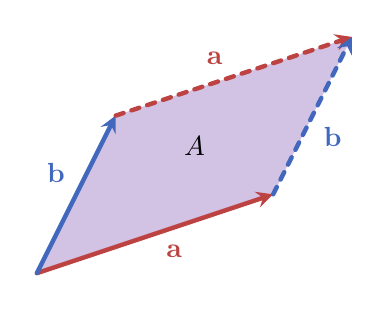
\begin{tikzpicture}
			\coordinate (a) at (3,1);
			\coordinate (b) at (1,2);
			\fill[xpurple!35] (0,0) -- (a) -- ++(b) -- (b) -- cycle;
			\node[fit={(0,0) (a) ($(a)+(b)$) (b)}] {$A$};
			\draw[vector={xred}]  (0,0) -- (a) node [midway, below right] {$\vec{a}$};
			\draw[vector={xblue}] (0,0) -- (b) node [midway, above left]  {$\vec{b}$};
			\draw[vector={xred}, dashed]  (b) -- ++(a) node [midway, above left]   {$\vec{a}$};
			\draw[vector={xblue}, dashed] (a) -- ++(b) node [midway, below right]  {$\vec{b}$};
		\end{tikzpicture}
	\end{center}
	\caption{The area of the parallelogram spanned by two vectors $\vec{a}$ and $\vec{b}$.}
	\label{fig:area_two_vecs}
\end{figure}

Let's check several properties of this area:
\begin{enumerate}
	\item The parallelogram spanned by the two basis vectors $\eb{1}$ and $\eb{2}$ has an area of $1$: $A\left(\eb{1},\eb{2}\right)=1$.
	\item If the two vectors are on the same line then the area equals $0$, i.e. $A\left(\vec{a}, \lambda\vec{a}\right)=0$, where $\lambda\in\Rs$.
	\item The parallelogram spanned by one vector $\vec{a}$ and a sum of two vectors $\vec{b}+\vec{c}$ has the same area as the sum of the areas of the two parallelograms spanned by $\vec{a},\ \vec{b}$ and by $\vec{a},\ \vec{c}$: $A\left(\vec{a},\vec{b}+\vec{c}\right)=A\left(\vec{a},\vec{b}\right)+A\left(\vec{a},\vec{c}\right)$ (\autoref{fig:adding_parallelograms}).
	\item Scaling any of the two vectors scales the area by the same factor: $A\left(\alpha\vec{a},\beta\vec{b}\right)=\alpha\beta A\left(\vec{a},\vec{b}\right)$, where $\alpha,\beta\in\Rs$ (\autoref{fig:scaling_parallelogram}). A special case of scaling is that of scaling by a negative scalar: for example, $A\left(-\vec{a},\vec{b}\right)=-A\left(\vec{a},\vec{b}\right)$.
\end{enumerate}

\begin{figure}
	\begin{center}
		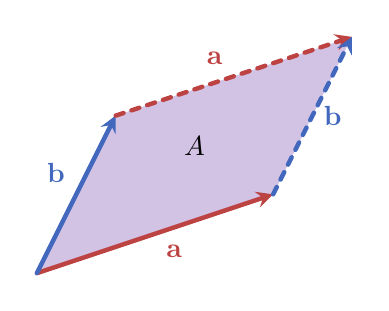
\begin{tikzpicture}
			\coordinate (a) at (3,1);
			\coordinate (b) at (1,2);
			\coordinate (c) at (0,2);
			\fill[xpurple!35] (0,0) -- (a) -- ++(b) -- (b) -- cycle;
			\node[fit={(0,0) (a) ($(a)+(b)$) (b)}] {$A$};
			\draw[vector={xred}]  (0,0) -- (a) node [midway, below right] {$\vec{a}$};
			\draw[vector={xblue}] (0,0) -- (b) node [midway, above left]  {$\vec{b}$};
			\draw[vector={xred}, dashed]  (b) -- ++(a) node [midway, above left] {$\vec{a}$};
			\draw[vector={xblue}, dashed] (a) -- ++(b) node [midway, right] {$\vec{b}$};
		\end{tikzpicture}
	\end{center}
	\caption{Adding two vectors\ldots}
	\label{fig:adding_parallelograms}
\end{figure}

\begin{figure}
	\begin{center}
		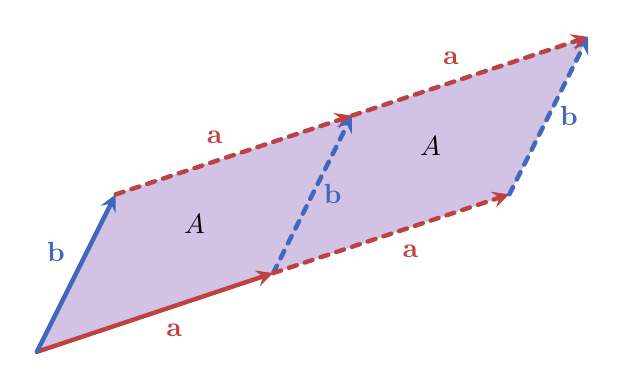
\begin{tikzpicture}
			\coordinate (a) at (3,1);
			\coordinate (b) at (1,2);
			\fill[xpurple!35] (0,0) -- ($2*(a)$) -- ++(b) -- (b) -- cycle;
			\node[fit={(0,0) (a) ($(a)+(b)$) (b)}] {$A$};
			\node[fit={(a) ($2*(a)$) ($2*(a)+(b)$) ($(a)+(b)$)}] {$A$};
			\draw[vector={xred}]  (0,0) -- (a) node [midway, below right] {$\vec{a}$};
			\draw[vector={xblue}] (0,0) -- (b) node [midway, above left]  {$\vec{b}$};
			\draw[vector={xred}, dashed]  (b) -- ++(a) node [midway, above left] {$\vec{a}$};
			\draw[vector={xblue}, dashed] (a) -- ++(b) node [midway, right] {$\vec{b}$};
			\draw[vector={xred}, dashed]  (a) -- ++(a) node [midway, below right] {$\vec{a}$};
			\draw[vector={xblue}, dashed] ($2*(a)$) -- ++(b) node [midway, right] {$\vec{b}$};
			\draw[vector={xred}, dashed]  ($(a)+(b)$) -- ++(a) node [midway, above left] {$\vec{a}$};
		\end{tikzpicture}
	\end{center}
	\caption{Scaling the vector $\vec{a}$ by a factor of $2$ scales the area of the parallelogram by the same factor.}
	\label{fig:scaling_parallelogram}
\end{figure}

Using the above properties, we can derive the relation between $A\left(\vec{a},\vec{b}\right)$ and $A\left(\vec{b},\vec{a}\right)$:
\begin{equation}
	\begin{aligned}
		A\left(\vec{a},\vec{b}\right) & = \cancel{A\left(\vec{a}+\vec{b},\vec{b}+\vec{a}\right)} - A\left(\vec{b},\vec{a}\right) \\
		                              & = -A\left(\vec{b},\vec{a}\right).
	\end{aligned}
	\label{eq:sqapping_order_of_vectors_area_paeallelogram}
\end{equation}
This means that swapping the order of vectors in the area of a parallelogram changes its sign.

\subsection{Matrix Rank and Null Space}

\section{Matrix-Matrix Products}

\section{Eigenvalues and Eigenvectors}

\end{document}
